\documentclass[a4paper,12pt]{article}
\usepackage[utf8]{inputenc}

% bib setup
\usepackage[authoryear]{natbib}
\setcitestyle{numbers,square}
% Bibliography style.
\bibliographystyle{plainnat}

\usepackage{graphicx}
\usepackage{framed}
\usepackage{listings,xcolor}
%\usepackage{inconsolata}

\definecolor{dkgreen}{rgb}{0,.6,0}
\definecolor{dkblue}{rgb}{0,0,.6}
\definecolor{dkyellow}{cmyk}{0,0,.8,.3}

\lstset{
  basicstyle=\ttfamily,
  columns=fullflexible,
  showstringspaces=false,
  commentstyle=\color{gray}\upshape,
  basicstyle=\small,
  numberstyle=\footnotesize,
  numbers=left,
  captionpos=b,
  stepnumber=1,
  numbersep=10pt,
  tabsize=2,
  breaklines=true,
}

\lstset{
  language        = php,
  basicstyle      = \small\ttfamily,
  keywordstyle    = \color{dkblue},
  stringstyle     = \color{red},
  identifierstyle = \color{dkgreen},
  commentstyle    = \color{gray},
  emph            =[1]{php},
  emphstyle       =[1]\color{black},
  emph            =[2]{if,and,or,else},
  emphstyle       =[2]\color{dkyellow}}

\title{Web Engineering: Miniproject}
\author{Jesper Riemer Andersen\\Nicklas Andersen\\Simon Reedtz Olesen}

\begin{document}
\maketitle

\section{Block 1: Introduction}
We have simple 3-tier architecture which allows us to communicate with the server and extract data from our database. This protects the database from unwanted queries from the client.

\begin{center}
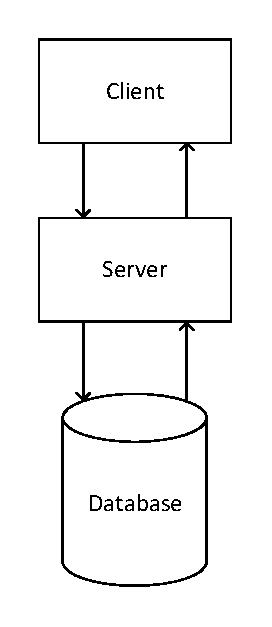
\includegraphics[scale=0.8]{3-tier.pdf}
\end{center}

\begin{enumerate}
\item The client opens his web browser and sends a HTTP request to the server.
\item The server runs the PHP script which queries data from the database.
\item The database returns the result according to the query.
\item Then the server returns the HTTP response to the client.
\item The response is then output as HTML.
\end{enumerate}

\begin{lstlisting}[language=php,label=lst:aspectratio] 
<?php
$connection = mysql_connect("localhost", "root", "");
mysql_select_db("webengi", $connection);

$query = mysql_query("SELECT testtext FROM hello", $connection);

while ($row = mysql_fetch_assoc($query)) {
    echo $row['testtext']."</br>";
}
?>
\end{lstlisting}

This code shows the steps explained above. We chose to run the server on localhost using WampServer, which also comes bundled with a MySQL database.

We start by connecting to the localhost with the username \textit{root} and empty password. Then we select the database called \textit{webengi}, and then query the database. For each row that is returned by the query, we echo the content of the column called \textit{testtext}.

\section{Block 2: Data I: XML etc.}

We found an XML document containing a small set of computers for sale on eBay, which we will display a subset of. We will be using the following:
\begin{itemize}
\item An XML file containing data on computers for sale.
\item An XSL file with our XSL transformations (XSLT).
\item A HTML file which contains only a little javascript to load the other files and display the result.
\end{itemize}

\begin{lstlisting}[language=xslt,label=lst:xslt] 
<?xml version="1.0" encoding="ISO-8859-1"?>
<xsl:stylesheet version="1.0" xmlns:xsl="http://www.w3.org/1999/XSL/Transform">

<xsl:template match="/">
  <h2>Computers for sale on eBay</h2>
    <table border="1">
      <tr bgcolor="#9acd32">
        <th>Current bid</th>
        <th>Memory</th>
        <th>Hard drive</th>
        <th>CPU</th>
      </tr>
      <xsl:for-each select="root/listing">
      <tr>
        <td><xsl:value-of select="auction_info/current_bid"/></td>
        <td><xsl:value-of select="item_info/memory"/></td>
        <td><xsl:value-of select="item_info/hard_drive"/></td>
        <td><xsl:value-of select="item_info/cpu"/></td>
      </tr>
      </xsl:for-each>
    </table>
</xsl:template>
</xsl:stylesheet>
\end{lstlisting}

This is the XSL file with our transformation. The following box is copied from w3schools.com \citep{w3xslt}.

\begin{framed}
Since an XSL style sheet is an XML document, it always begins with the XML declaration: \lstinline$<?xml version="1.0" encoding="ISO-8859-1"?>$.

The next element, \lstinline$<xsl:stylesheet>$, defines that this document is an XSLT style sheet document (along with the version number and XSLT namespace attributes).

The \lstinline$<xsl:template>$ element defines a template. The \lstinline$match="/"$ attribute associates the template with the root of the XML source document.

The content inside the \lstinline$<xsl:template>$ element defines some HTML to write to the output.
\end{framed}

\bibliography{bibliografi}
\end{document}